% !TeX spellcheck = de_CH
% !TeX encoding = UTF-8
% !TeX root = ../presentation.tex

\section{Gegenmassnahmen}

\begin{frame}{Was genau ist $F(c)$?}
\begin{itemize}
\item Ergibt sich aus thermodynamischen,
sowie chemischen Eigenschaften
\item Ändert sich \glqq sprunghaft\grqq{} um eine Temperatur $T_\text{krit}$
\end{itemize}
\begin{figure}
\centering
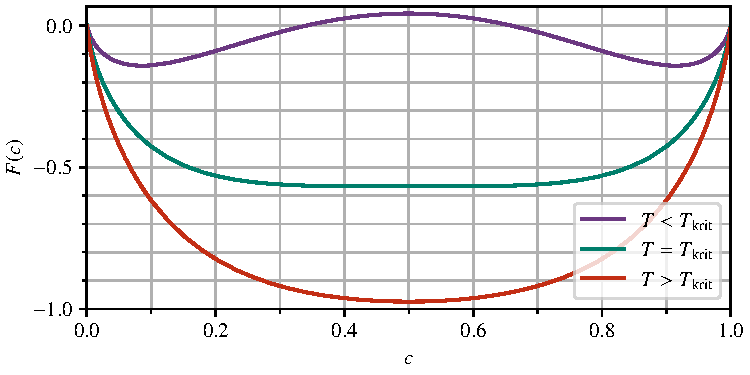
\includegraphics[scale=0.8]{images/energy}
\caption{Temperaturabhängigkeit von $F(c)$}
\label{fig:fc}
\end{figure}
\end{frame}

\begin{frame}{Gegenmassnahmen}
\begin{enumerate}
\item<+-> Erhitzen über kritische Temperatur $T_\text{krit}$
\uncover<+->{$\rightarrow$ eher ungeeignet für Salatsaucen}
\item<+-> Verwenden eines Emulgators (z. B. Senf, Eier, Honig, \ldots)
\item<+-> Verwenden eines Stabilisators (z. B. Xanthan, Agar-Agar, \ldots)
\item<+-> Intensives Rühren
\end{enumerate}
\end{frame}

\begin{frame}{Rühren}
\begin{itemize}
\item Hinzufügen eines inkrompessiblen Strömungsfeld $v(x, t)$.
Dadurch erhält der Fluss $\flux$ eine zusätzliche Komponente:
\begin{align*}
\pderiv{c}{t} + v \cdot \nabla c
&=
\nabla \cdot (M \nabla \mu)
\\
\mu
&=
\deriv{F}{c} -  \epsilon^2 \Delta c
\\
\nabla \cdot v
&=
0
\end{align*}
\item Hinzufügen von periodischen Randbedingungen
\begin{alignat*}{2}
v_x(x, y, t)
&=
\alpha \sin(y + \phi_n)
,\quad&
& n \tau \leq t < (n+1) \tau
\\
v_y(x, y, t)
&=
\alpha \sin(x + \psi_n)
,&
& n \tau \leq t < (n+1) \tau
\end{alignat*}
\end{itemize}
\end{frame}

% \begin{frame}{}
% \begin{figure}
% \centering
% \foreach \i in {0.1,0.3,0.5,0.7,1.0}{
% \begin{subfigure}{0.19\textwidth}
% \centering
% \includegraphics[width=\textwidth]{images/\i.png}
% \caption{$\alpha = \i$}
% \end{subfigure}
% }
% \begin{subfigure}{0.19\textwidth}
% \centering
% 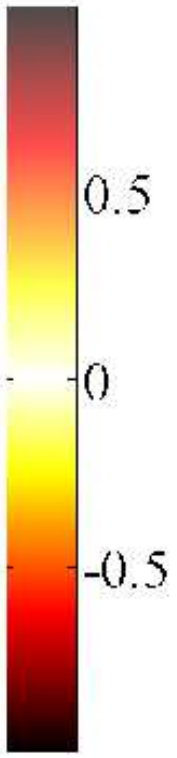
\includegraphics[width=0.2\textwidth]{images/cb.png}
% \caption{Farbskala}
% \end{subfigure}
% \caption{Resultate nach langem Rühren für unterschiedliche Amplituden $\alpha$ {\color{mainColor}[1]}}
% \end{figure}
% \end{frame}

\begin{frame}{Anfangsbedingung}
\begin{figure}
\centering
\begin{subfigure}{0.32\textwidth}
\centering

\includegraphics[width=\textwidth]{images/ach_sim/initial.pdf}
\caption{Anfangsbedingung $c(x,0)$}
\end{subfigure}
%
\begin{subfigure}{0.32\textwidth}
\centering
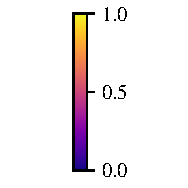
\includegraphics[width=0.8\textwidth]{images/colorbar}
\caption{Farbskala}
\end{subfigure}
\caption{Anfangsbedingung $c(x,0)$ der Simulation}
\end{figure}
\end{frame}

\begin{frame}{}
\begin{figure}
\centering
%
% \begin{subfigure}{0.19\textwidth}
% \centering
% 
\includegraphics[width=\textwidth]{images/ach_sim/initial.pdf}
% \caption{$c(x,0)$}
% \end{subfigure}
%
\begin{subfigure}{0.32\textwidth}
\centering
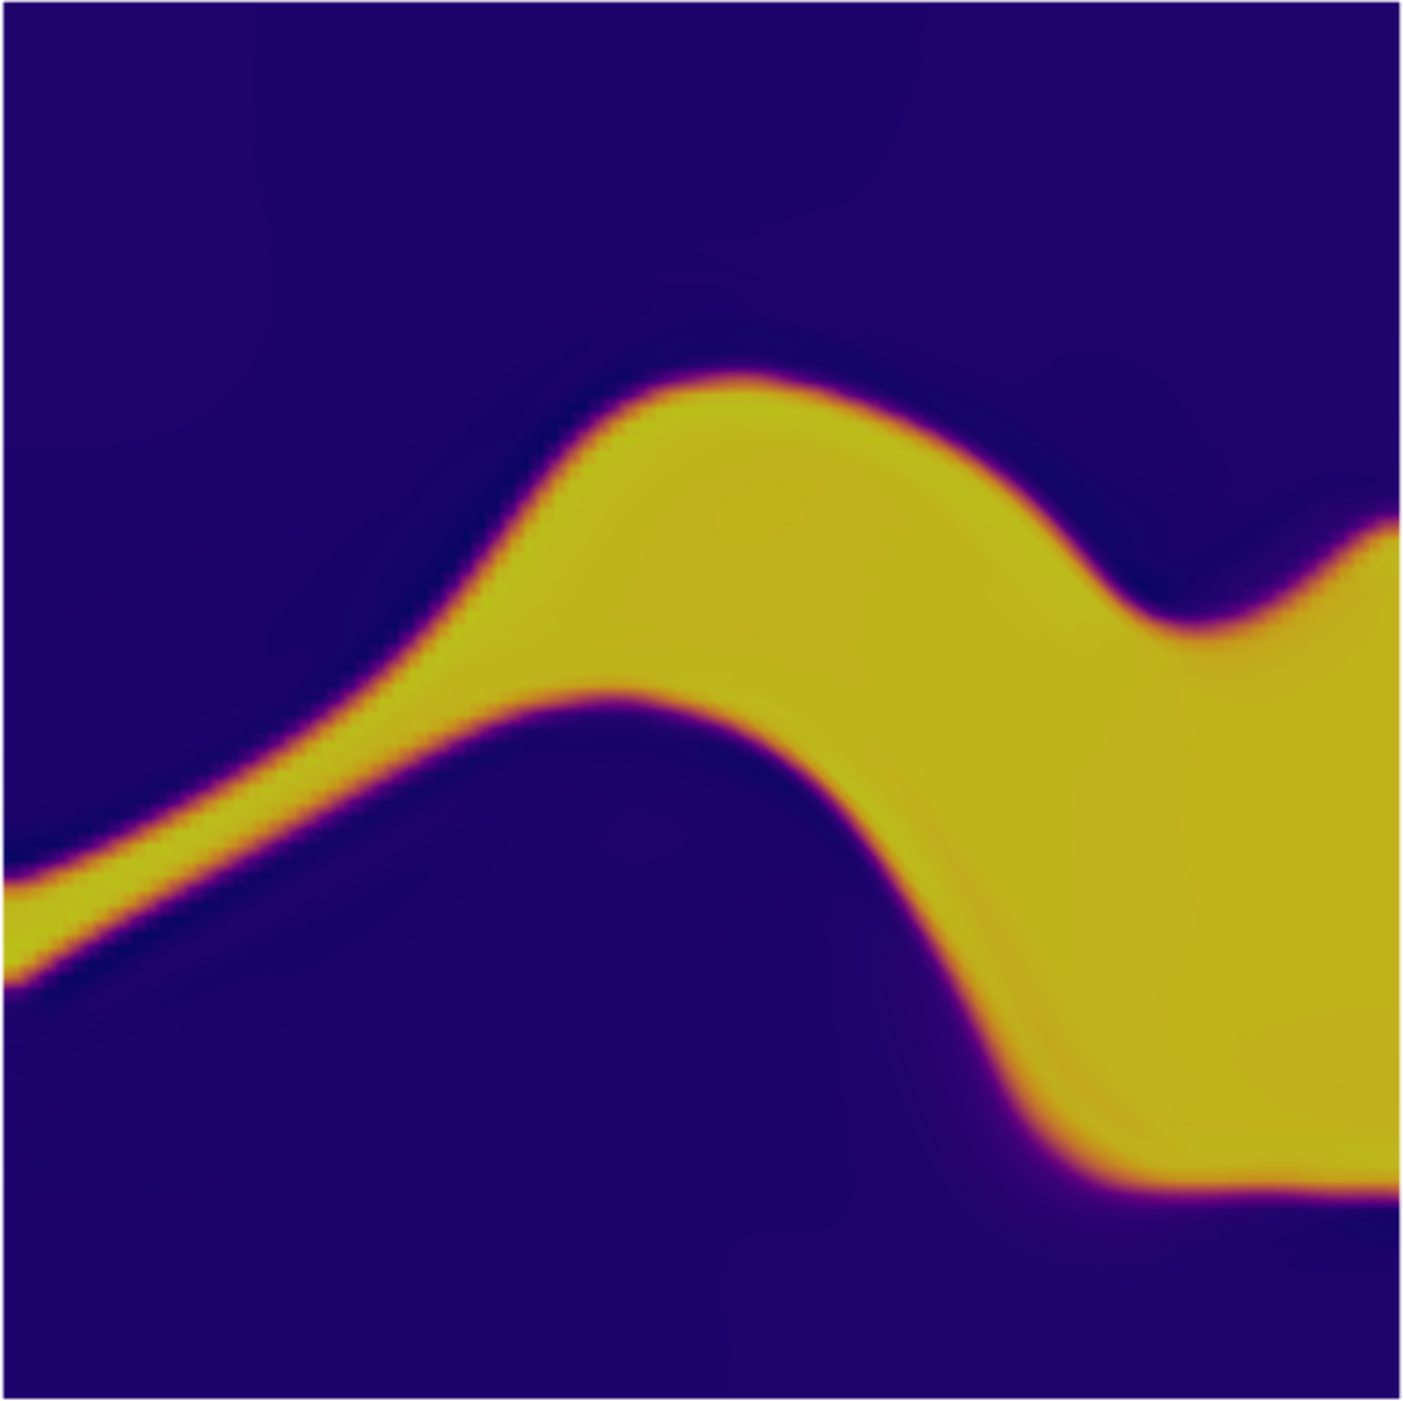
\includegraphics[width=\textwidth]{images/ach_sim/very_weak.pdf}
\caption{$\alpha$ sehr klein}
\end{subfigure}
%
\begin{subfigure}{0.32\textwidth}
\centering
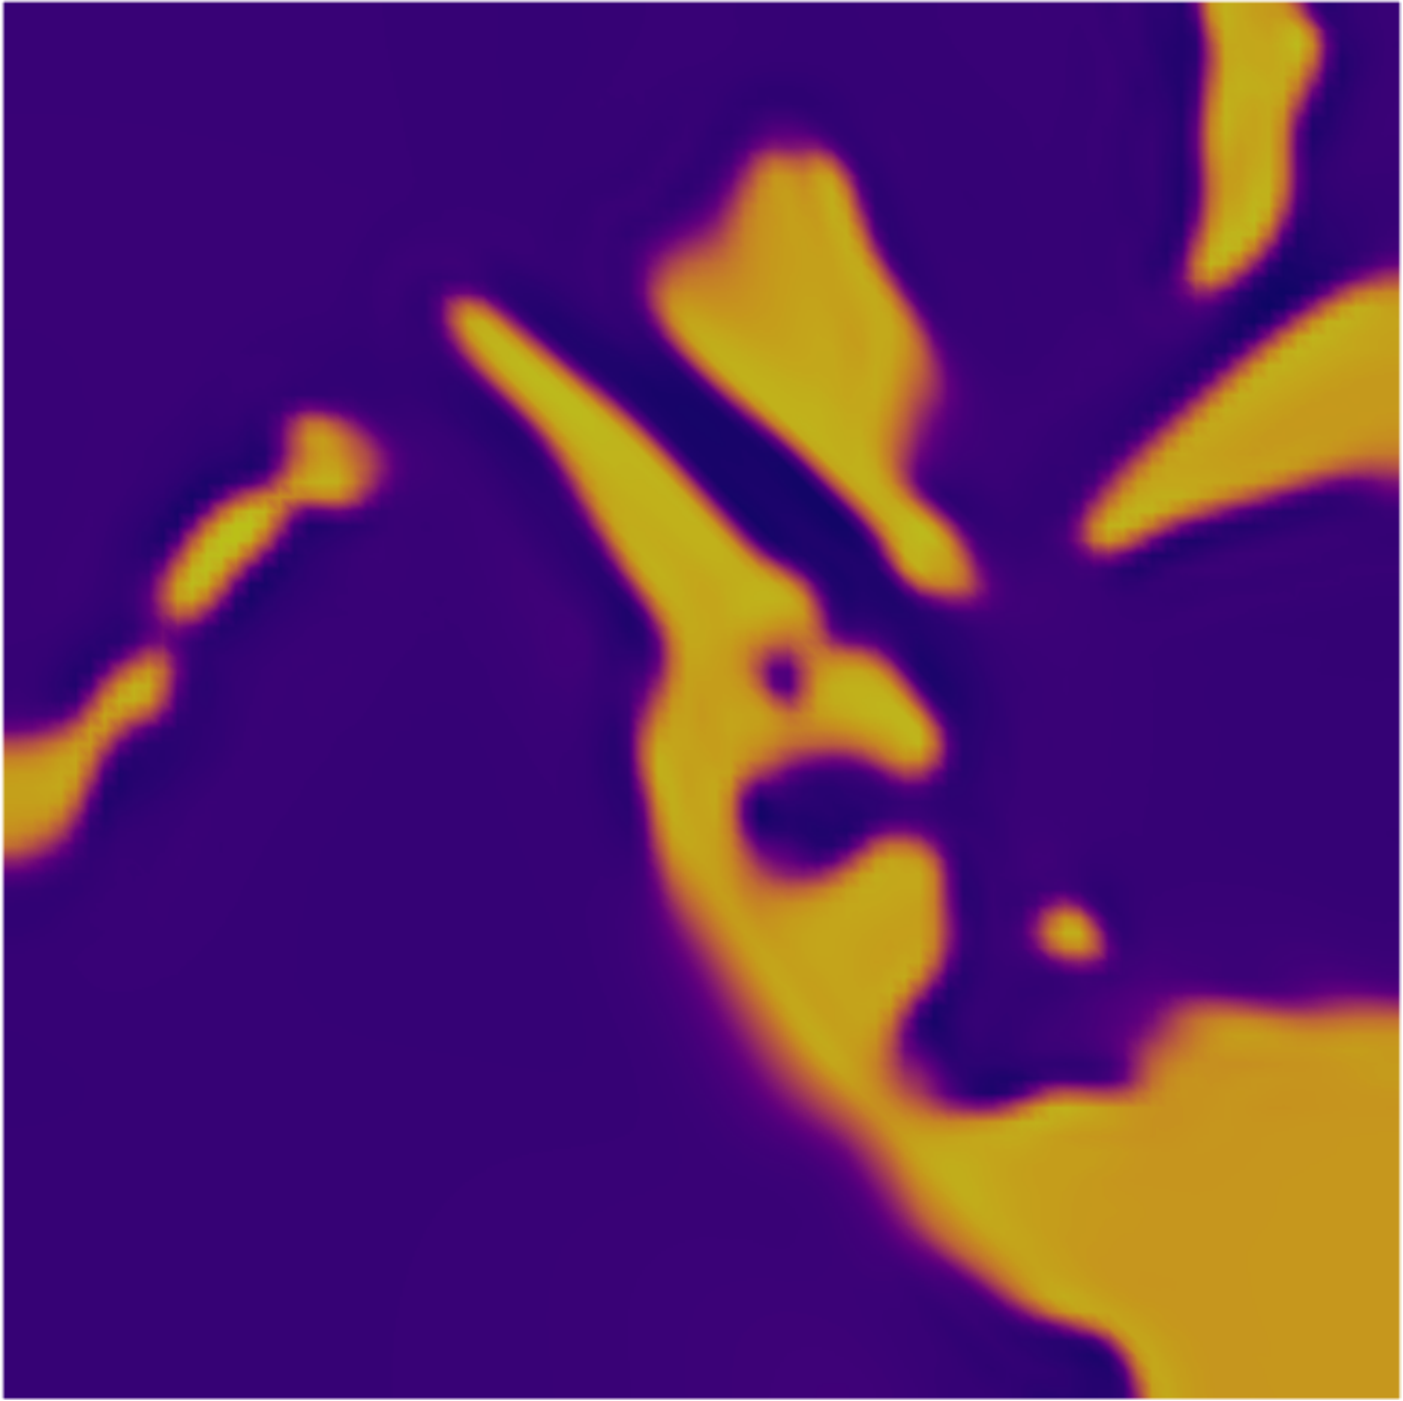
\includegraphics[width=\textwidth]{images/ach_sim/weak.pdf}
\caption{$\alpha$ klein}
\end{subfigure}
%
\begin{subfigure}{0.32\textwidth}
\centering
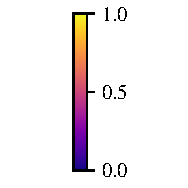
\includegraphics[width=0.8\textwidth]{images/colorbar}
\caption{Farbskala}
\end{subfigure}
\caption{Resultate nach langem Rühren $c(x,1000\tau)$
für unterschiedliche Amplituden $\alpha$}
\end{figure}
\end{frame}


\begin{frame}
\begin{figure}
\centering
\begin{subfigure}{0.32\textwidth}
\centering
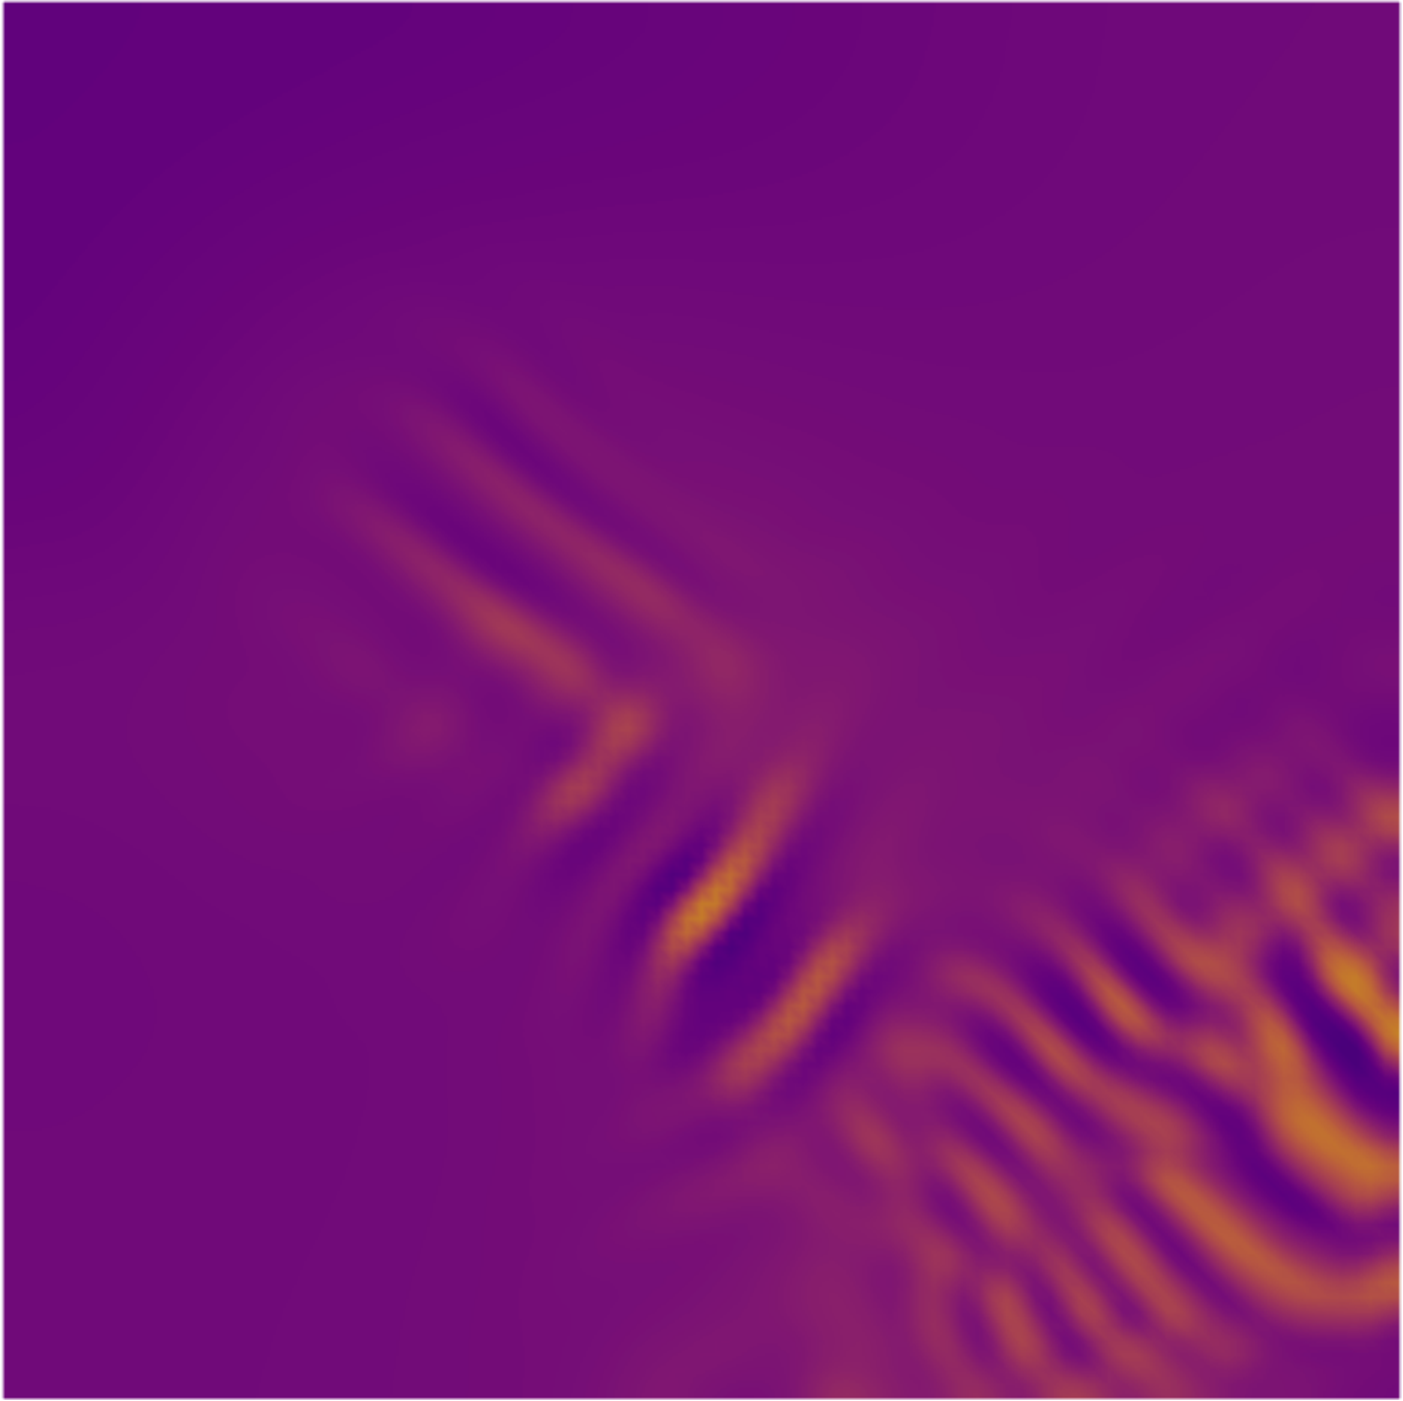
\includegraphics[width=\textwidth]{images/ach_sim/nearly.pdf}
\caption{$\alpha$ moderat}
\end{subfigure}
%
\begin{subfigure}{0.32\textwidth}
\centering

\includegraphics[width=\textwidth]{images/ach_sim/strong.pdf}
\caption{$\alpha$ gross}
\end{subfigure}
%
\begin{subfigure}{0.32\textwidth}
\centering
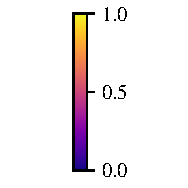
\includegraphics[width=0.8\textwidth]{images/colorbar}
\caption{Farbskala}
\end{subfigure}
\caption{Resultate nach langem Rühren $c(x,1000\tau)$ für unterschiedliche Amplituden $\alpha$ }
\end{figure}

\end{frame}
